\documentclass[11pt, a4paper, spanish]{article}

\usepackage[a4paper, margin=2.5cm, top=3.5cm, bottom=3.5cm]{geometry} % Define los márgenes
\usepackage{amsmath, amscd, amssymb, amsthm, latexsym, gensymb} % Paquetes matemáticos
\usepackage[spanish]{babel} % Traduce los paquetes a español
\usepackage[utf8]{inputenc} % Codificación UTF8
\usepackage{fancyhdr} % Encabezados y pies de página
    \pagestyle{fancyplain}
\usepackage{enumerate}
\usepackage{xspace}
\usepackage[page, toc]{appendix} % Apéndices
\usepackage[nottoc]{tocbibind} % Referencias en la TDC
\usepackage{scrextend} % Para usar addmargin
\usepackage{listings} % Código
    \lstdefinestyle{customcpp}{
        belowcaptionskip=1\baselineskip,
        breaklines=true,
        xleftmargin=3em,
        language=C++,
        basicstyle=\small\ttfamily
    }
\usepackage[onelanguage, spanish]{algorithm2e}
    % \NoCaptionOfAlgo
    \LinesNumbered\RestyleAlgo{ruled}\IncMargin{1em}\DontPrintSemicolon\SetArgSty{}\SetCommentSty{textsf}\SetFuncSty{textsf}
    \SetKwProg{For}{para}{ hacer}{fin}
    \SetKwProg{Fn}{función}{:}{fin}
\usepackage[pdftex]{graphicx} % Imágenes
\usepackage[usenames,dvipsnames]{color} % Autoexplicativo
\usepackage{caption} % Captions sin números
\usepackage{multirow}
\usepackage{caratula} % Carátula del DC
\usepackage{url}

% Bibliografía
\usepackage{biblatex}
\addbibresource{referencias.bib}

% Comandos personalizados
\let\strong\textbf
\renewcommand{\appendixtocname}{Apéndices}
\renewcommand{\appendixpagename}{Apéndices}
\theoremstyle{plain}
    \newtheorem{prop}{Proposición}
    \newtheorem{lema}{Lema}
\theoremstyle{remark}
    \newtheorem{obs}{Observación}
\setlength{\parskip}{.3em}
\newcommand{\acr}[1]{\textsc{\lowercase{#1}}} % Acrónimos
\newcommand{\mat}[1]{\ensuremath{\mathbf{#1}}} % Matrices

% Encabezado
\lhead{Métodos Numéricos}
\rhead{Trabajo Práctico Nº 2 - \emph{``Ohhh solo tiran $\pi$-edras\dots''}}
% Pie de pagina
\renewcommand{\footrulewidth}{0.4pt}
% \lfoot{FCEN}
% \rfoot{UBA}

\begin{document}

% Datos de carátula
\materia{Métodos Numéricos}
\titulo{Trabajo Práctico Nº 2}
\subtitulo{``Ohhh solo tiran $\pi$-edras\dots''}
\fecha{Segundo cuatrimestre de 2015}

\integrante{Frizzo, Franco}{013/14}{francofrizzo@gmail.com}
\integrante{Martínez, Manuela}{160/14}{martinez.manuela.22@gmail.com}
\integrante{Rabinowicz, Lucía}{105/14}{lu.rabinowicz@gmail.com}

% Carátula
\maketitle
\newpage

% Resumen y palabras clave
\begin{addmargin}[4em]{4em}

\section*{\centering Resumen}

En este trabajo, se busca solucionar dos problemas sobre elaboración de \emph{rankings}: la clasificación de páginas web para ordenar los resultados de un motor de búsqueda en Internet, y la de equipos según su desempeño en ligas deportivas. Para resolverlos, se presentarán los algoritmos \emph{PageRank} y \emph{GeM}, respectivamente. Ambos proporcionan una solución representando los datos en forma matricial y buscando luego el autovector principal de esta matriz. Se realizan pruebas experimentales sobre estos métodos, variando sus parámetros de entrada, y comparándolos con algoritmos alternativos en términos de eficiencia y efectividad.

\vspace{4em}
\noindent \strong{Palabras clave:} \emph{PageRank}, motores de búsqueda, \emph{rankings} deportivos, cálculo de autovectores

\end{addmargin}
\clearpage

% Índice
\tableofcontents
\clearpage

% Contenido
\section{Introducción}

    En la actualidad, Internet ocupa un lugar central en la vida cotidiana de millones de personas, y una de las principales tareas que estas llevan a cabo en línea es la búsqueda de información. A eso se debe el rol central que ocupan los buscadores, y la gran importancia de contar con algoritmos que permitan indexar y clasificar la información disponible en la red y, muy especialmente, seleccionar de este enorme volumen de datos solo aquellos que sean más relevantes para un determinado contexto de búsqueda.

    Por otro lado, las partidos de las grandes ligas deportivas movilizan a enormes masas de seguidores a lo largo y a lo ancho de todo el mundo, y además, importantes intereses económicos dependen de sus resultados. Por lo tanto, es de gran interés que estos resultados puedan definirse con criterios justos y objetivos, que no sea preseten a la especulación y sean robustos ante posibles intentos de manipulación.

    Si bien a primera vista estos dos problemas pueden parecer poco relacionados, poseen características en común: en ambos casos, se busca dar un orden de importancia a una determinada colección de elementos, organizándolos en un \emph{ranking} en base información estadística que puede obtenerse sobre las relaciones existentes entre ellos.

    En este trabajo, se introducirá uno de los métodos que ha sido utilizado con gran éxito para resolver el primero de los problemas mencionados: el algoritmo de \emph{PageRank}, presentado en 1998 por Sergey Brin y Larry Page\cite{Brin1998}, que constituye una parte esencial del motor del reconocido buscador Google. Tras una introducción teórica a los conceptos matemáticos que fundamentan este método, se presentará una implementación del mismo y se expondrán resultados experimentales con el fin de analizar su eficiencia y su capacidad para resolver el problema planteado.

    Por otra parte, y de forma paralela, se procederá a abordar la situación planteada por el problema de la clasificación de equipos en ligas deportivas. Se mostrará que, tal y como se expone en Govan et al.\cite{Govan2008}, \emph{PageRank} puede ser adaptado sin mayores dificultades para emplearse como criterio de clasificación en este contexto, y se analizará el caso particular de su utilización para elaborar la tabla de posiciones del torneo de Primera Divisón de la Asociación del Fútbol Argentino (AFA), realizando experimentos para evaluar su desempeño en comparación con el sistema de puntajes actual, y la forma en la que su funcionamiento ve afectado por variaciones en los parámetros del algoritmo.

        \subsection{Conceptos teóricos}

        En esta sección, enunciamos a modo introductorio los principales conceptos que funcionan como sustento teórico de los métodos numéricos que emplearemos. Nuestro objetivo no es profundizar en los mismos, dado que ya existen excelentes trabajos realizados que abordan cada uno de ellos más en detalle.

        Consideremos un sistema que puede tomar diferentes estados, dentro de un conjunto finito de ellos. Un \emph{proceso estocástico} es una sucesión de estos estados. Si consideramos un caso particular de proceso estocástico, en que la probabilidad de que el sistema se encuentre en un estado dado en el momento $k+1$ queda completamente determinada por su estado en el momento $k$, tenemos una \emph{cadena de Márkov}.

        Supongamos que el sistema tiene $n$ estados posibles, y denominemos $p_{ij}$ a la probabilidad de que el sistema pase del estado $j$ al estado $i$. Entonces podemos acomodar estos valores en una matriz $P \in \mathbb{R}^{n \times n}$, que llamaremos \emph{matriz de transición} de la cadena.

        Notemos que todas las entradas de la matriz, dado que indican valores de una probabilidad, son no negativas, y además, para $j = 1, \cdots, n$, tenemos que $\sum_{i=1}^{n} p_{ij} = 1$. A una matriz que cumpla con estas condiciones la denominaremos \emph{matriz estocástica por columnas}, y, como enuncian Bryan y Leise en \cite{Bryan2006}, cumplen con la importante propiedad de tener a $1$ como autovalor dominante; es decir, $1$ es autovalor y además, para cualquier otro $\lambda \in \mathbb{R}$ autovalor de una de estas matrices, se cumple que $|\lambda| < 1$. Si, además, una matriz estocástica cumple que todas sus entradas son estrictamente positivas, entonces podemos afirmar que el espacio de autovectores asociados al autovalor $1$ tiene dimensión $1$.

        En este trabajo, será de interés para nosotros poder calcular este autovector. Se cuentan con métodos muy diversos para realizarlo, pero muchos de ellos son excesivamente costosos, especialmente cuando las matrices son de dimensiones considerables. Afortunadamente, para matrices con las características que acabamos de mencionar, el autovector principal puede calcularse mediante un método iterativo, muy sencillo de formular, conocido como \emph{método de la potencia}. Este método se basa en el siguiente resultado: si $x$ es el autovector principal de la matriz $A$, y $v$ es un vector inicial cualquiera, entonces $\lim_{k\to\infty}A^k v = x$. Es decir, partiendo de un vector inicial y multiplicando repetidas veces por la matriz $A$, el resultado eventualmente convergerá al autovector buscado. Para una demostración de este hecho, como así también una exposición más detallada del proceso, puede consultarse \cite{Kamvar}[Section 3]. Como podrá verse en la sección siguiente, y comprobarse luego experimentalmente, este algoritmo resulta muy apropiado para resolver los problemas planteados en este trabajo, y es capaz de aprovechar características propias de las matrices con las que trataremos para mejorar su eficiencia.

\clearpage
\section{Desarrollo}

    \subsection{Conceptos teóricos}

        En esta sección, enunciamos a modo introductorio los principales conceptos que funcionan como sustento teórico de los métodos numéricos que emplearemos. Nuestro objetivo no es profundizar en los mismos, dado que ya existen excelentes trabajos realizados que abordan cada uno de ellos más en detalle.

        Consideremos un sistema que puede tomar diferentes estados, dentro de un conjunto finito de ellos. Un \emph{proceso estocástico} es una sucesión de estos estados. Si consideramos un caso particular de proceso estocástico, en que la probabilidad de que el sistema se encuentre en un estado dado en el momento $k+1$ queda completamente determinada por su estado en el momento $k$, tenemos una \emph{cadena de Márkov}.

        Supongamos que el sistema tiene $n$ estados posibles, y denominemos $p_{ij}$ a la probabilidad de que el sistema pase del estado $j$ al estado $i$. Entonces podemos acomodar estos valores en una matriz $\mat{P} \in \mathbb{R}^{n \times n}$, que llamaremos \emph{matriz de transición} de la cadena.

        Notemos que todas las entradas de la matriz, dado que indican valores de una probabilidad, son no negativas, y además, para $j = 1, \cdots, n$, tenemos que $\sum_{i=1}^{n} p_{ij} = 1$. A una matriz que cumpla con estas condiciones la denominaremos \emph{matriz estocástica por columnas}, y, como enuncian Bryan y Leise en \cite{Bryan2006}, cumplen con la importante propiedad de tener a $1$ como autovalor dominante; es decir, $1$ es autovalor y además, para cualquier otro $\lambda \in \mathbb{R}$ autovalor de una de estas matrices, se cumple que $|\lambda| < 1$. Si, además, una matriz estocástica cumple que todas sus entradas son estrictamente positivas, entonces podemos afirmar que el espacio de autovectores asociados al autovalor $1$ tiene dimensión $1$.

        En este trabajo, será de interés para nosotros poder calcular este autovector. Se cuentan con métodos muy diversos para realizarlo, pero muchos de ellos son excesivamente costosos, especialmente cuando las matrices son de dimensiones considerables. Afortunadamente, para matrices con las características que acabamos de mencionar, el autovector principal puede calcularse mediante un método iterativo, muy sencillo de formular, conocido como \emph{método de la potencia}. Este método se basa en el siguiente resultado: si $x$ es el autovector principal de una matriz $\mat{A}$, y $v$ es un vector inicial cualquiera, entonces $\lim_{k\to\infty}\mat{A}^k v = x$. Es decir, partiendo de un vector inicial y multiplicando repetidas veces por la matriz $\mat{A}$, el resultado eventualmente convergerá al autovector buscado. Para una demostración de este hecho, como así también una exposición más detallada del proceso, puede consultarse \cite[Sección 3]{Kamvar2003}. Como podrá verse en la sección siguiente, y comprobarse luego experimentalmente, este algoritmo resulta muy apropiado para resolver los problemas planteados en este trabajo, y es capaz de aprovechar características propias de las matrices con las que trataremos para mejorar su eficiencia.

    \subsection{Métodos utilizados}

        \subsubsection{\emph{PageRank}: autovectores para elaborar un \emph{ranking} de páginas web}

        Cualquier usuario de Internet que haya realizado alguna búsqueda en Google habrá notado que, en la inmensa mayoría de los casos, la información deseada no se encuentra demasiado lejos de los primeros resultados arrojados por el buscador. ¿Cómo es clasificada la ingente cantidad de datos disponibles en la Web para lograr presentar al usuario aquellos que tienen mayor relevancia? El punto clave reside en aprovechar la información que cada página web brinda acerca de las demás a través de los vínculos o \emph{links} existentes entre ellas. La idea en que se basa el criterio adoptado es simple: cuantas más páginas tengan \emph{links} que apunten hacia otra página dada, más alta será la probabilidad de que esta última contenga información relevante; y mucho más lo será si los enlaces provienen de orígenes que son, a su vez, considerados importantes.

        La World Wide Web, como cualquier otra red de páginas unidas a través de enlaces, puede ser considerada como un grafo dirigido, con las primeras representadas por los nodos y los segundos, por las aristas. Como punto de partida para elaborar el \emph{ranking}, recurriremos a una versión modificada de la matriz de adyacencia de este grafo, donde para cada página el peso de los enlaces salientes será inversamente proporcional a su cantidad. Denotemos $n_{j}$ a la cantidad de \emph{links} salientes que posee la página $j$, y $L_i$ al conjunto de páginas que poseen un link que apunta hacia $i$. Entonces, si llamamos $\mat{A}$ a esta matriz, tenemos que $a_{ij} = \frac{1}{n_{j}}$ si $j \in L_i$, y $a_{ij} = 0$ en caso contrario.

        Nuestro objetivo es calcular un \emph{ranking} $x = (x_1, \cdots, x_n)$, donde $x_i$ es el puntaje asignado a la página $i$. Una manera de hacerlo siguiendo el criterio antes mencionado es planteando el sistema de ecuaciones
        \[ x_i = \sum_{j \in L_i} \frac{x_j}{n_j} \qquad i = 1, \cdots n \]

        Notemos que este sistema corresponde a la representación matricial $\mat{A}x = x$. Es decir, el problema se reduce a encontrar un autovector de $\mat{A}$ asociado al autovalor $1$. ¿Podemos garantizar la existencia de una solución a este sistema, y en tal caso, su unicidad?

        Analizando la matriz $\mat{A}$, podemos notar que, por un lado, $0 \leq a_{ij} \leq 1 (\forall\ i, j)$, y por otra parte, si $n_j > 0$, entonces $\sum_{i=1}^{n} a_{ij} = 1$, y si, por el contrario, $n_j = 0$, entonces $\sum_{i=1}^{n} a_{ij} = 0$. Conceptualmente, cuando una página tiene \emph{links} salientes, los pesos de los mismos suman $1$, mientras que las columnas cuyos valores suman $0$ corresponden a las páginas que no tienen enlaces salientes (o \emph{nodos colgantes}). Por lo tanto, si consideramos una red sin nodos colgantes, tenemos que $\mat{A}$ es una matriz estocástica por columnas; esto garantiza la existencia de un autovector asociado al autovalor $1$ y, nos dice, además, que cualquier otro autovalor $\lambda$ de $\mat{A}$ deberá cumplir $|\lambda| < 1$. El modelo construido representa un proceso de Márkov; como explican Brin y Page\cite{Brin1998}, este puede interpretarse como el itinerario de un \emph{navegante aleatorio}, que posicionado en una página $j$ cualquiera, se dirige a cualquiera de sus links con probabilidad $\frac{1}{n_j}$.

        Para resolver el problema de los nodos colgantes, consideramos que cuando el navegante llega a uno de estos nodos, selecciona equiprobablemente una página cualquiera de la red para continuar su recorrido. Matematicamente esto puede representarse con una nueva matriz $\mat{P_1} = \mat{A} + \mat{D}$, donde $\mat{D} = v d^t$, con

        \begin{center}\begin{tabular}{ccc}
            $\displaystyle v_i = \frac{1}{n}$ & \qquad y & \qquad $d_i = \begin{cases} 1 & \text{si }n_i = 0 \\ 0 & \text{si no} \end{cases}$
        \end{tabular}\end{center}

        $\mat{P_1}$ sí es una matriz estocástica por columnas, lo cual nos asegura que encontraremos solución. Más aún, dado que $1$ es el autovalor principal de $\mat{P_1}$, sabemos que podremos hacerlo aplicando el método de la potencia. Ahora bien, es altamente deseable que la solución hallada sea única, para que las páginas queden clasificadas de manera única. Con el sistema tal y como está planteado, no es difícil encontrar ejemplos en los que existe más de una solución posible (ver \cite{Bryan2006}). Afortunadamente, esto también se resuelve de manera sencilla mediante el agregado al modelo de un \emph{factor de amortiguación} o \emph{teletransportación}\footnote{El nombre \emph{factor de teletransportación} hace referencia aque, desde la interpretación del navegante aleatorio antes mencionada, la alteración que se efectúa al sistema puede interpretarse como agregarle la posibilidad de que en cada paso, con probabilidad $c$, el navegante se ``teletransporte'' a una página elegida al azar, independientemente de la existencia de un \emph{link} que conecte esta con su posición actual.} $c$, $0 < c < 1$, que permite definir

        \[ \mat{P_2} = c \mat{P_1} + (1 - c) \mat{E} \]

        \noindent donde $\mat{E} \in \mathbb{R}^{n \times n}$ tiene $\frac{1}{n}$ en todas sus posiciones. Notemos que, dado que $\mat{P_1}$ y $\mat{E}$ son matrices estocásticas por columnas, $\mat{P_2}$, que es un promedio ponderado de ambas, también lo es; y que, además, $\mat{P_2}$ tiene todos sus coeficientes estrictamente positivos. Es decir, $\mat{P_2}$ representa una cadena de Márkov ergódica, y por lo tanto, el sistema $\mat{P_2} x = x$ tiene solución única.

        \subsubsection{\emph{GeM}: adaptando \emph{PageRank} para clasificar equipos en ligas deportivas}

        El algoritmo presentado en la sección anterior no solo ha resultado sumamente exitoso para resolver el problema para el que fue ideado; también existen otros problemas que pueden resolverse con la misma idea básica. Como ya mencionamos anteriormente, uno de ellos es la elaboración de \emph{rankings} de equipos para ligas deportivas a partir de los resultados obtenidos en los partidos.

        En Govan et al.\cite{Govan2008}, los autores mencionan algunos métodos empleados para este fin, y los comparan frente a uno desarrollado por ellos mismos: \emph{GeM}, que está fuertemente basado en el algoritmo de \emph{PageRank}. La idea es la siguiente: una temporada de una liga deportiva también puede entenderse como un grafo dirigido. Los nodos representan a los equipos, y una arista entre los nodos $i$ y $j$ quiere decir que el equipo $i$ perdió al menos una vez contra el equipo $j$. El peso de las aristas es proporcional a la diferencia absoluta en el marcador del partido al que representan (la suma de ellas, si se trata de más de un partido), normalizadas de forma tal que la suma de los pesos de todas las aristas salientes de cada nodo sea igual a $1$.

        A partir del grafo anteriormente mencionado, puede construirse la matriz $\mat{A}$ de adyacencia del grafo; y, de la misma manera que en el caso de la clasificación de páginas en buscadores, pueden derivarse de ella las matrices $\mat{P_1}$ y $\mat{P_2}$ para resolver los problemas de los nodos colgantes (que representan, en este caso, a los equipos invictos) y de la posible existencia de más de una solución. El sistema resultante es completamente análogo al obtenido para calcular \emph{PageRank}, por lo que no detallaremos los pormenores matemáticos que permiten encontrar su solución. Sí deben tenerse en cuenta las inevitables diferencias implementativas que se derivarán de los distintos contextos de uso en los que se desempeñarán ambos algoritmos, que trataremos con más profundidad en la próxima sección.

    \subsection{Implementación}

    Ambos métodos fueron implementados en lenguaje C++, reutilizando el código en los casos en que fue posible, pero atendiendo a las diferencias en los contextos de aplicación esperados para cada uno, especialmente a la hora de decidir las estructuras de datos utilizadas.

    En los dos casos, una vez leídos los datos de entrada, se crea la matriz correspondiente al sistema a resolver. A continuación, partiendo de un vector de probabilidad uniforme ($v \in \mathbb{R}^n$, con $v_i = \frac{1}{n}$ para $i = 1, \cdots, n$), se aplican sucesivas iteraciones del método de la potencia. Como criterio de detención, se estima la convergencia del método en cada iteración; para esto, se calcula la diferencia Manhattan entre el vector obtenido en cada repetición y en la inmediatamente anterior, y se la compara con un umbral de tolerancia, proporcionado como parámetro al momento de la ejecución. El algoritmo se detiene cuando la distancia obtenida está por debajo del umbral.

        \subsubsection{Implementación de \emph{PageRank}}

        En el caso del algoritmo \emph{PageRank}, se tuvieron especialmente en cuenta dos hechos: por un lado, el contexto de uso hace esperar que deban manejarse enormes cantidades de datos, por lo que es importante hacer hincapié en la eficiencia de la implementación; por otra parte, en una red con una estructura similar a la de la World Wide Web, cabe esperar que la cantidad de links presentes en cada página sea muy escasa en comparación con el número total de páginas. Esto permite optimizar la forma en la que se almacena la información: en particular, la matriz $\mat{A}$ correspondiente al sistema, que contiene los datos sobre los \emph{links} de la red, es \emph{esparsa}, es decir, gran parte de sus coeficientes son $0$. Dado que las alteraciones posteriores de esta matriz (las efectuadas a fin de solucionar el problema de los nodos colgantes y el de las posibles múltiples soluciones), a partir de las cuales se obtiene la matriz $\mat{P_2}$, pueden ser aplicadas \emph{ad-hoc} al momento de operar, se decidió aprovechar la ventaja mencionada y limitarse a almacenar en memoria la matriz $\mat{A}$.

        La representación elegida fue \acr{CSC} (\emph{Compressed Sparse Column}). Esta representación consiste en tres vectores. El primero de ellos (\texttt{vals}) almacena todos los valores no nulos de la matriz, recorriéndola por columnas; el segundo (\texttt{ind\_filas}), de igual longitud que el primero, contiene el índice de la fila en que se encuentra el elemento respectivo en \texttt{vals}; el tercero (\texttt{ptr\_cols}), tiene una entrada por columna, y señala en qué posición de \texttt{vals} se encuentra el primer valor correspondiente a cada una de ellas. Esta representación fue elegida por sobre \acr{DOK} (\emph{Dictionary of Keys}) por considerarla más eficiente, tanto en memoria como temporalmente, y por sobre \acr{CSR} (\emph{Compressed Sparse Row}) porque permite distinguir eficientemente las columnas que solo contienen ceros (que requieren en este caso un tratamiento especial): en la presente implementación, se las representa colocando el valor $-1$ en la posición correspondiente del vector \texttt{ptr\_cols}.

        El único inconveniente que se encontró con la representación elegida es que resulta muy impráctica a la hora de cargar los datos. Es por eso que como paso intermedio entre la lectura de datos y la creación de la matriz, se utilizó una estructura temporal que se asemeja más al formato de \acr{DOK}: un vector correspondiente a las columnas, cuyas entradas son a su vez vectores conteniendo los índices de la columna respectiva donde deberá colocarse un valor no nulo.

        La implementación del método de la potencia no presentó grandes complicaciones: consiste en un ciclo que inicia con un vector con todas sus componentes iguales a $\frac{1}{n}$ y lo multiplica, en cada iteración, por la matriz del sistema. Implementar este producto implicó algo más de complejidad, ya que la matriz por la que se debe multiplicar es diferente a la almacenada en memoria. La multiplicación se realiza columna a columna, siguiendo el orden natural de la estructura elegida para la matriz. Se utiliza un vector acumulador para calcular el resultado, que se inicializa con todas sus posiciones en $0$. Luego, para $i = 1, \cdots, n$, se utiliza la matriz $\mat{A}$ para calcular el producto entre la columna $i$ de la matriz $\mat{P_2}$ por el valor $v_i$ del vector de entrada, y el resultado se suma al vector acumulador. Para cada columna pueden presentarse dos casos, que deben tratarse de forma distinta:

        \begin{enumerate}
            \item Si la columna $i$ de $\mat{A}$ solo contiene valores nulos (es decir, \texttt{ptr\_cols[i-1]} = \texttt{-1}), tendremos que, para todo $j = 1, \cdots, n$, ${p_2}_{ij} = c (\frac{1}{n}) + (1-c) (\frac{1}{n}) = \frac{1}{n}$. Luego, el producto de esta columna por $v_i$ puede calcularse directamente, y será un vector con todas sus componentes iguales a $\frac{v_i}{n}$.
            \item Si, por el contrario, en la columna $i$ de $\mat{A}$ hay valores no nulos, para $j = 1, \cdots, n$, tendremos que ${p_2}_{ij} = c (a_{ij}) + (1-c) (\frac{1}{n})$. Es decir, el producto de esta columna por $v_1$ puede calcularse en dos pasos: primero, consideramos un vector con todas sus componentes iguales a $(1-c) (\frac{1}{n})$, y luego, para los índices $j$ tales que $a_{ij} \neq 0$, le sumamos $c (a_{ij})$ a la componente correspondiente de dicho vector.
        \end{enumerate}

        \subsubsection{Implementación de \emph{GeM}}

        La implementación del método \emph{GeM} fue considerablemente más simple, debido a que, si bien ya no es válida la hipótesis de que la matriz obtenida será esparsa, sí puede asumirse que la instancias a tratar serán considerablemente menores. Dado que el algoritmo es básicamente el mismo, gran parte del código de \emph{PageRank} pudo reutilizarse; las principiales modificaciones estuvieron en la forma de representación de la matriz y, por consiguiente, en la implementación del producto de esta con un vector.

        Para el almacenamiento de la matriz, se decidió utilizar un vector de vectores (cada uno de estos representando una fila de la matriz), por considerar que brindaba un equilibrio adecuado entre eficiencia y facilidad de implementación. Dado que ahora se guardan en memoria todos los coeficientes, se decidió almacenar $\mat{P_2}$ en lugar de $\mat{A}$. De esta forma, las operaciones que transforman la segunda en la primera solo se hacen una vez, durante la carga de los datos, y se incrementa la simplicidad y la eficiencia de la función encargada de calcular el producto entre la matriz y el vector. Esta última función opera ahora de la forma tradicional, multiplicando cada fila de $\mat{P_2}$ por el vector proporcionado y almacenando el resultado en la componente correspondiente del resultado.

\clearpage
\section{Experimentación}

	\subsection{\emph{PageRank} y páginas web}

	A continuación, se presentan los experimentos que se realizaron. Con el código del trabajo práctico se incluye una serie de scripts de \emph{bash} que permiten recrear los experimentos realizados, como así también los gráficos que se incluyen en este informe; esto puede hacerse ingresando al directorio \texttt{exp} dentro de la raíz, y ejecutando el comando \texttt{./exp{i}.sh}, siendo \texttt{i} el número de experimento.

		\subsubsection{Experimento 1}
			\subsubsection*{Presentación}
			En el primer experimento se quiere observar como varía el tiempo de ejecución a medida que se modifica el valor del parámetro $c$, para lograr que la norma Manhattan entre dos iteraciones consecutivas sea menor que la tolerancia indicada. Para ello se toma una determinada cantidad de páginas web que no se modificarán a lo largo del experimento y se ejecutará el programa para diferentes valores de $c$. Con el fin de mejorar la precisión de los resultados y evitar posibles interferencias (por ejemplo, las generadas por otras tareas que pueda estar ejecutando la computadora) cada medición se repitió 10 veces, tomando luego el promedio de los datos obtenidos

			\subsubsection*{Hipótesis}
			Se conjetura que cuanta mayor sea la probabilidad de teletransportarse de una página a otra, menos tiempo va a tardar el algoritmo en llegar al estado en el que la tolerancia sea menor que la norma Manhattan. $(1-c)$ indica cuál es la probabilidad de, estando en cualquier página, teletransportarse a otra. Por esto es que cuanto más chico sea el valor de $c$, menos tiempo de ejecución demorará el algoritmo.

			\subsubsection*{Datos de entrada} 
			Se toman 13 páginas con 16 \emph{links}. Además el parámetro $c$ toma los valores \texttt{0, 0.1, 0.2, 0.3, 0.4, 0.5, 0.6, 0.7, 0.8, 0.9, 1}. La tolerancia es de \texttt{0.00001}. Se eligió la cantidad de páginas y el valor de la tolerancia arbitrariamente, procurando que los casos de prueba no fueran excesivamente grandes para no prolongar innecesariamente la duración de las pruebas. 

			\subsubsection*{Resultados}
				{\centering \begin{tabular}{c}
			      % 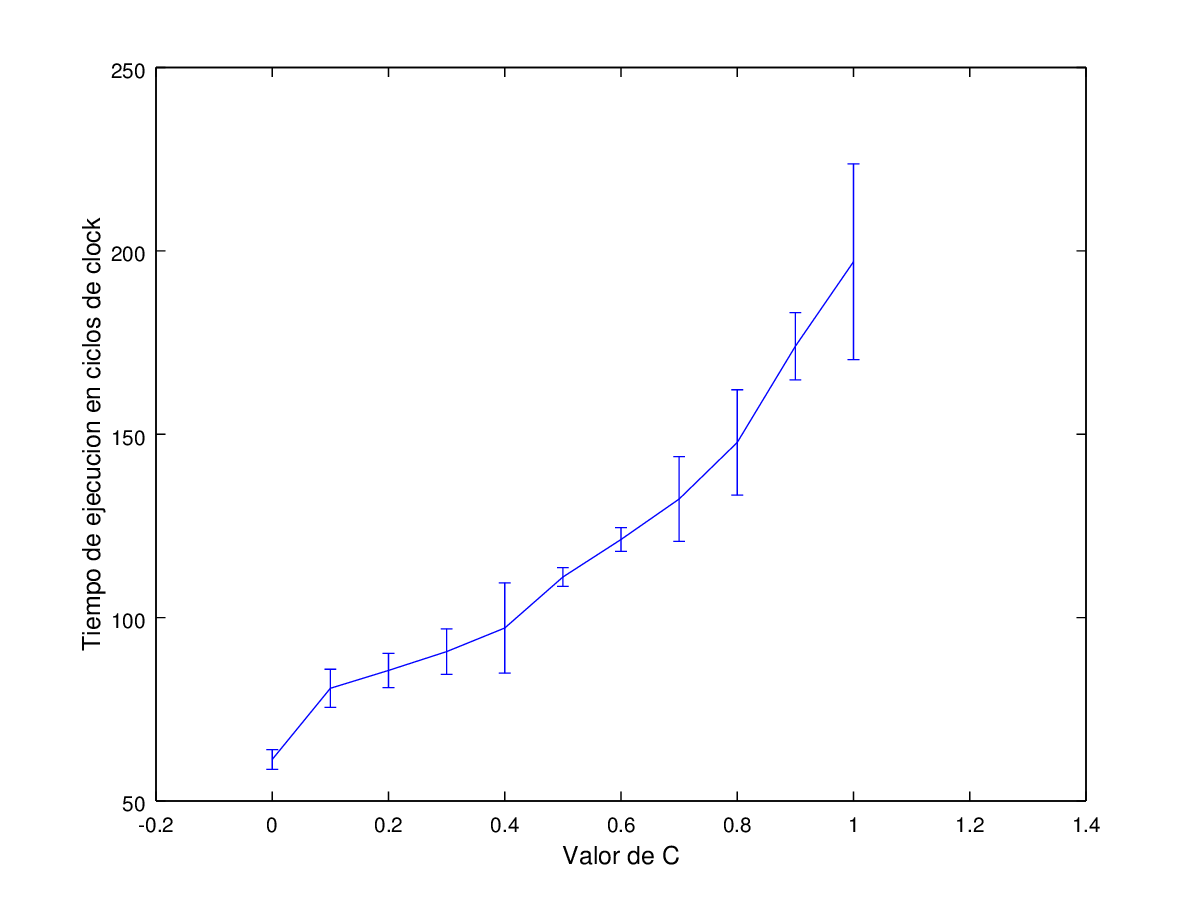
\includegraphics[width=12cm]{../../src/exp/graficos/exp1.png} \\
			    \end{tabular}}

			\subsubsection*{Discusión} 
			Como se puede observar en el experimento, a medida que aumenta el valor de c, aumenta el tiempo de ejecución. Esto se debe a que la matriz inicial no es homogénea y la que formamos a partir del c si lo es. Así, cuando la segunda toma dicha importancia, el sistema tiende más rápido a ser homogéneo y requiere menos iteraciones del ciclo para lograr una norma menor a la tolerancia deseada. 


		\subsubsection{Experimento 2}
			\subsubsection*{Presentación}
			Con este experimento se pretende observar la diferencia en el tiempo de ejecución cuando se varía la cantidad de \emph{links} en una determinada cantidad de páginas, manteniendo el valor de la tolerancia constante.
			Para ello se utilizan listas de páginas diferentes como parámetro de entrada en cada una de las ejecuciones a comparar, pero manteniendo la cantidad de las mismas. Se toma el tiempo que se demora en ejecutar el algoritmo y se lo divide por la cantidad de iteraciones realizadas. Esto permite obtener un promedio del tiempo que demora por cada una de las iteraciones del ciclo.
		
			\subsubsection*{Hipótesis} 
			Suponemos que variar la cantidad de \emph{links} altera más el tiempo de ejecución que variar la cantidad de páginas sin que estén relacionadas entre ellas. Esto se debe a que, dada la forma en la que está implementado el algoritmo, sacando provecho del hecho de que la matriz es esparsa, agregar entradas a la matriz de adyacencia tendrá un mayor impacto sobre la cantidad de operaciones a realizar. Por lo tanto, se espera observar que el tiempo de ejecución aumente a medida que la cantidad de relaciones entre páginas sea mayor.

			\subsubsection*{Datos de entrada} 		
			Para este experimento se toman 50 páginas. La cantidad de \emph{links} entre ellas varía, tomando los valores \texttt{4, 32, 70, 105, 130, 160}. Estos valores fueron elegidos a modo de análisis. Para generarlos se creó una red a partir de diferentes páginas web interconectadas entre sí. Luego se borraron algunas páginas, eliminando una determinada cantidad de \emph{links}, y se agregaron nuevas páginas desconectadas totalmente de las ya existentes. De esta forma, no se disminuyó la cantidad de páginas pero sí la de \emph{links}. Además el valor de $c$ es \texttt{0.85} y el valor de la tolerancia es \texttt{0.00001}. El valor de $c$ y de la tolerancia fueron elegidos arbitrariamente, procurando que los casos de prueba no fueran excesivamente grandes para no prolongar innecesariamente la duración de las pruebas. 
			
			\subsubsection*{Resultados}
				{\centering \begin{tabular}{c}
			      % 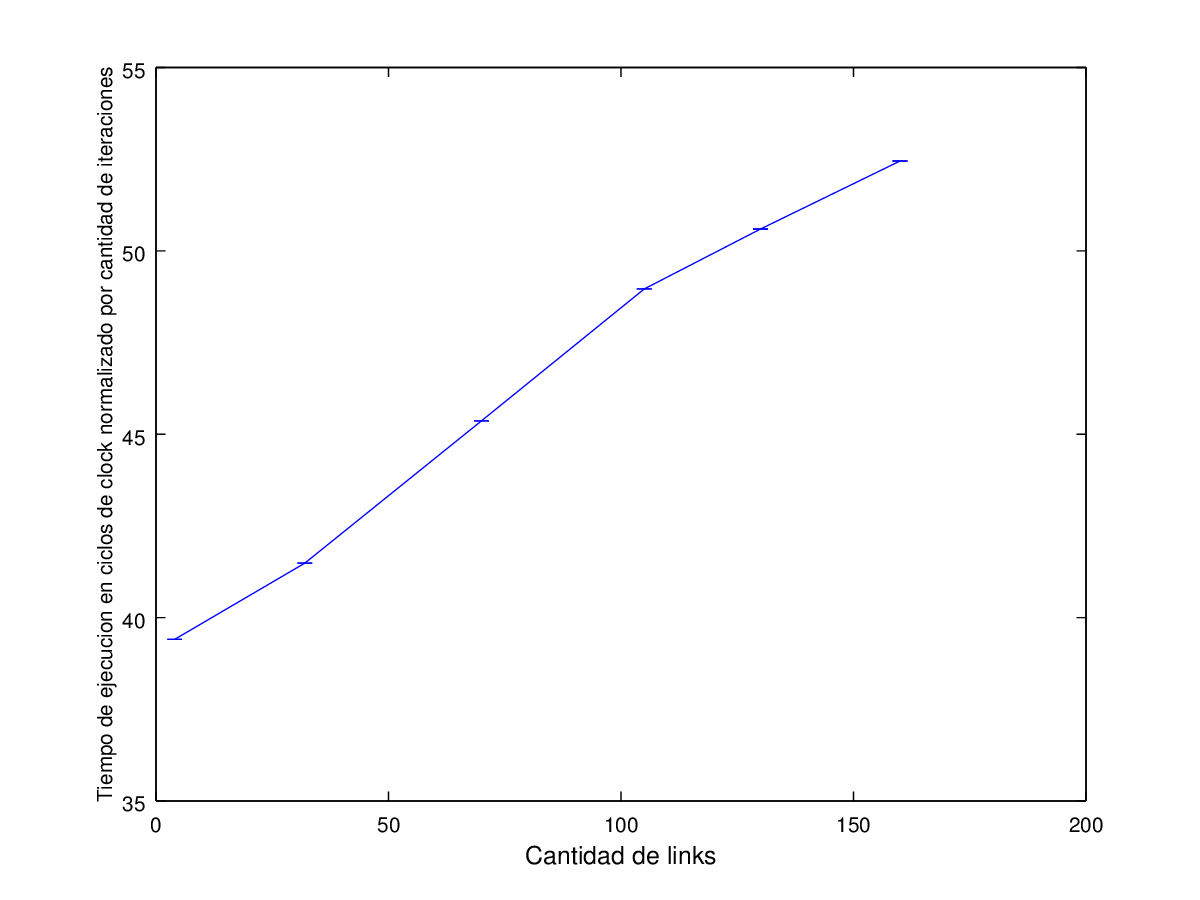
\includegraphics[width=12cm]{../../src/exp/graficos/exp2.png} \\
			    \end{tabular}}


			\subsubsection*{Discusión}
			Como se puede observar en el gráfico, a medida que aumentan las relaciones entre las páginas el tiempo de ejecución es mayor.  

		\subsubsection{Experimento 3}
			\subsubsection*{Presentación}
			En este experimento también se observa la diferencia en el tiempo de ejecución, pero comparando igual cantidad de páginas y relaciones entre las mismas y variando el valor de la tolerancia.
			Para ello se toma como parámetro de entrada en cada una de las ejecuciones una misma lista de páginas y se incrementa el valor de la tolerancia.

			\subsubsection*{Hipótesis} 
			Creemos que cuanto mayor sea la tolerancia, menor será el tiempo de ejecución del algoritmo. Esto se debe a que el algoritmo termina cuando la diferencia Manhattan es menor que la tolerancia. Entonces cuanto más grande sea el valor de la tolerancia, más rápido se cumplirá la condición para salir del ciclo y menos tardará en ejecutarse el algoritmo. Suponemos que para los valore mas chicos de tolerancia el tiempo de ejecución será altamente mayor que para valores de tolerancia cercanos a 1. Es decir, el crecimiento será exponenecial a medida que disminuimos el valor de la tolerancia.

			\subsubsection*{Datos de entrada} 
			Se toman 13 páginas con 16 \emph{links}. Además la tolerancia toma los siguientes valores: \texttt{0.000001, 0.000005, 0.00001, 0.00005, 0.0001, 0.0005, 0.001, 0.005, 0.01, 0.1, 0.3, 0.5, 0.7}. El parámetro $c$ es igual a \texttt{0.85}. El valor de $c$ y la cantidad de páginas fueron elegidos arbitrariamente, procurando que los casos de prueba no fueran excesivamente grandes para no prolongar innecesariamente la duración de las pruebas. Los valores de la tolerancia fueron tomados a modo de análisis teniendo en cuenta que el objetivo del experimento. 

			\subsubsection*{Resultados}
				{\centering \begin{tabular}{c}
			      % 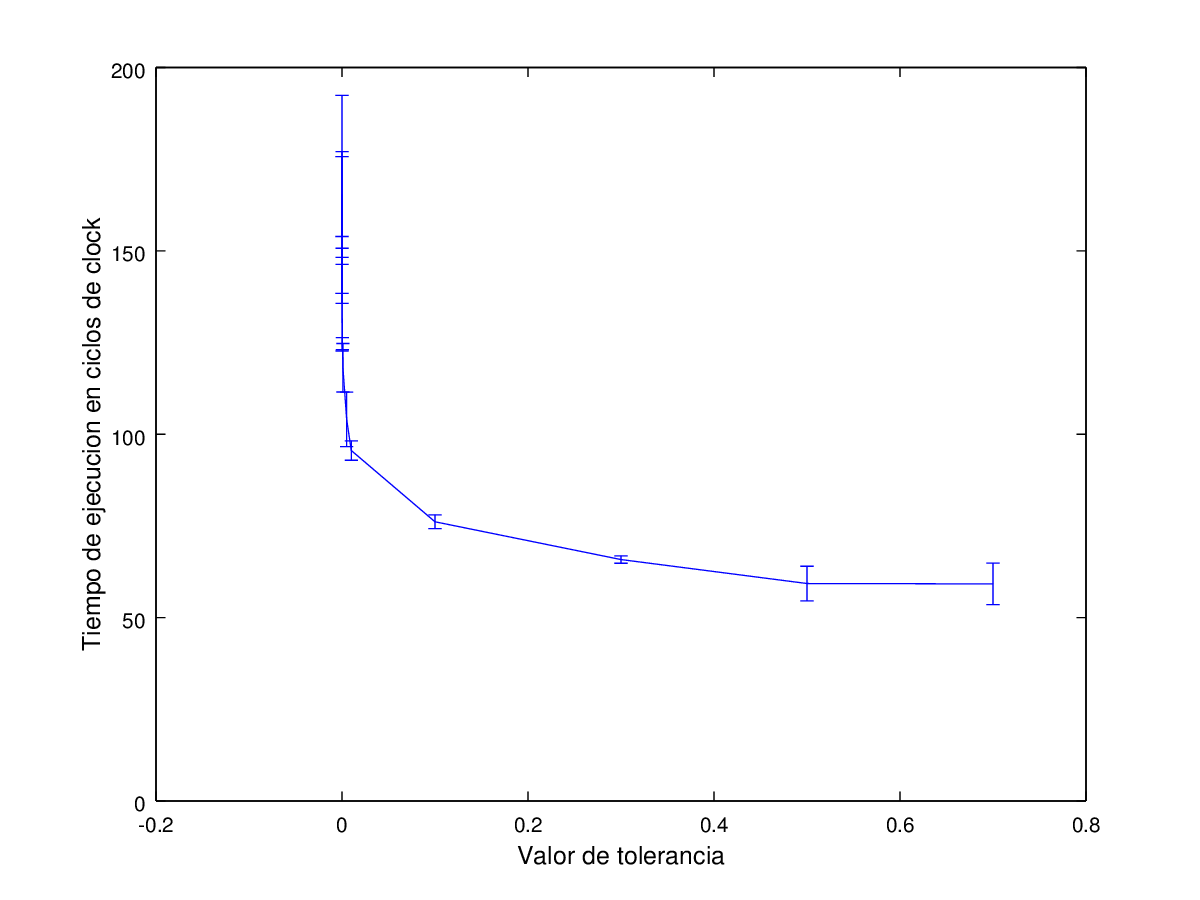
\includegraphics[width=12cm]{../../src/exp/graficos/exp3.png} \\
			    \end{tabular}}

			\subsubsection*{Discusión}
			Como se puede ver en el gráfico, al aumentar la tolerancia disminuye el tiempo de ejecución linealmente. Al estar en escala logaritmica, esto quiere decir que la función decrece de forma exponencial. Para valores de tolerancia cercanos a 1, la cantidad de iteraciones a realizar es notoriamente menor que para valores de tolerancia cercanos a 0. Esto sucede ya que el método converge cada vez mas lento, entonces cuando la tolerancia toma valores muy chicos las ultimas iteraciones modifican muy poco el vector por lo que se requieren más iteraciones para acercarse al resultado.
			Además se puede observar que hasta el valor de tolerancia 0.01 la variación en tiempo de ejecución dependiendo del valor de la tolerancia es mínimo. Cuando ese valor es menor que 0.01 el tiempo de ejecución se incrementa notoriamente. Dejamos a experimentos futuros ver cuál es el valor en el que el tiempo de ejecución es muy grande. En este sentido, se pudo confirmar la hipótesis.   

	\subsubsection{Experimento 4}
		\subsubsection*{Presentación}
		Otra de las pruebas consiste en comparar los \emph{rankings} formados al ejecutar los algoritmos de \emph{PageRank} y el de \textsc{In-deg}. Primero se analiza una lista de páginas de entrada en la que una de ellas sea apuntada por el resto (Web 1). 

		Luego se realiza la comparación con una lista en la que hayan dos páginas (a las que llamaremos página 1 y página 3) que sean apuntadas por varias paginas. Además, la página 3 tendrá un link a la 1. También se cuenta con otra (a la que llamaremos página 2) que apunta y es apuntada por la página 1, tal como se muestra en el siguiente esquema (Web 2):

			\begin{figure}[h]

				\begin{center}
					\begin{tabular}{@{\extracolsep{2cm}} cc}
				      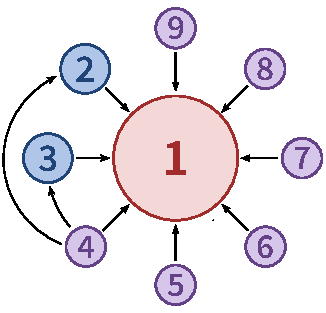
\includegraphics{imagenes/exp4-graph1.pdf} & 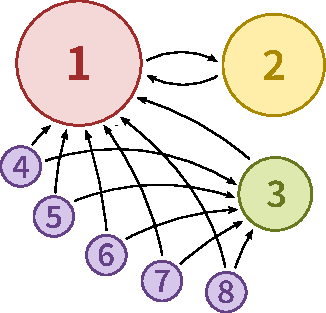
\includegraphics{imagenes/exp4-graph2.pdf} \\
				      {\small \strong{Web 1}} & {\small \strong{Web 2}}
				    \end{tabular}
			    \end{center}

		    	\caption{Redes utilizadas como datos de entrada para el Experimento 4} \label{fig:exp4-webs}

		    \end{figure}

			\subsubsection*{Hipótesis} 
			En el primero, suponemos que los \emph{rankings} obtenidos en ambos casos serán iguales ya que existe una sola página principal y el resto tiene igual cantidad de relaciones. Por otro lado, en el segundo notaremos diferencias. Llamaremos enlace fuerte a aquel que va de una página que es apuntada por muchas otras hacia otra página. El método \emph{PageRank} tiene en cuenta cuál es el peso de los \emph{links} que apuntan a las distintas páginas. En el caso de \textsc{In-deg}, solo se utiliza como información la cantidad de enlaces que llegan a cada una de las distintas páginas.

			En el experimento, si consideramos el método \emph{PageRank}, la página 1 quedará en primer lugar, ya que es la que recibe más \emph{links} a la misma, pero en segundo lugar quedará la página 2. Esto se debe a que el enlace de la 1 a la 2 es un enlace muy fuerte. En el caso de \textsc{In-deg}, esto no sucede ya que este método solo toma en cuenta que existe un único link hacia la página 2. Por lo tanto en \emph{PageRank} las posiciones serán 1-2-3 y luego el resto. En \textsc{In-deg} tendremos primero a la página 1 seguida de la 3, luego la 2 y finalmente el resto.

			\subsubsection*{Datos de entrada}
			Para la Web 1, se tomaron 9 páginas con 10 \emph{links}. Para la Web 2, se tomaron 8 páginas con 13 \emph{links}.  

			El valor de $c$ es \texttt{0.85} y el valor de tolerancia es \texttt{0.00001}. 
			 		
			\subsubsection*{Resultados}

			   \begin{center}
	      			\begin{tabular}{c|c|c} 
			      		\hline
			  				\multicolumn{3}{c}{\emph{Ranking} Web 1 - \emph{PageRank}} \\
			 			\hline
	        			Posición & Nodo & Puntaje \\ \hline
	         			1 & 1 & 0.473848 \\
	        			2 & 8 & 0.078821 \\
	        			3 & 9 & 0.078821 \\
	        			4 & 2 & 0.061418 \\
	        			5 & 3 & 0.061418 \\
	        			6 & 4 & 0.061418 \\
	        			7 & 5 & 0.061418 \\
	        			8 & 6 & 0.061418 \\
	        			9 & 7 & 0.061418 
	      			\end{tabular} 

	      			\begin{tabular}{c|c|c}
			      		\hline
			  				\multicolumn{3}{c}{\emph{Ranking} Web 1 - \textsc{In-deg}} \\
			 			\hline
	        			Posición & Nodo & Puntaje \\ \hline
	         			1 & 1 & 0.8 \\
	        			2 & 8 & 0.1 \\
	        			3 & 9 & 0.1 \\
	        			4 & 2 & 0 \\
	        			5 & 3 & 0 \\
	        			6 & 4 & 0 \\
	        			7 & 5 & 0 \\
	        			8 & 6 & 0 \\
	        			9 & 7 & 0 
	      			\end{tabular}

	      			\begin{tabular}{c|c|c}
			      		\hline
			  				\multicolumn{3}{c}{\emph{Ranking} Web 2 - \emph{PageRank}} \\
			 			\hline
	        			Posición & Nodo & Puntaje \\ \hline
	         			1 & 1 & 0.448059 \\
	        			2 & 2 & 0.448059 \\
	        			3 & 3 & 0.058594 \\
	        			4 & 4 & 0.058594 \\
	        			5 & 5 & 0.018750 \\
	        			6 & 6 & 0.018750 \\
	        			7 & 7 & 0.018750 \\
	        			8 & 8 & 0.018750
	      			\end{tabular}
	    		
	      			\begin{tabular}{c|c|c}
			      		\hline
			  				\multicolumn{3}{c}{\emph{Ranking} Web 2 - \textsc{In-deg}} \\
			 			\hline
	        			Posición & Nodo & Puntaje \\ \hline
	         			1 & 1 & 0.538462 \\
	        			2 & 3 & 0.384615 \\
	        			3 & 2 & 0.076923 \\
	        			4 & 4 & 0 \\
	        			5 & 5 & 0 \\
	        			6 & 6 & 0 \\
	        			7 & 7 & 0 \\
	        			8 & 8 & 0 \\
	      			\end{tabular}
	    	\end{center}

			\subsubsection*{Discusión} 
			Como podemos ver en los \emph{rankings} del primer análisis en ambos casos quedan iguales. En cambio, en el segundo observamos variaciones, ya que en la lista de entrada el peso de todos los enlaces no es el mismo, es decir, hay enlaces más fuertes que otros. A diferencia de \emph{PageRank}, el método \textsc{In-deg} no tiene en cuenta esta propiedad. Por lo tanto, si en las páginas de entrada todos los \emph{links} tienen igual fuerza, el resultado obtenido por ambos métodos no difiere. 


	\subsection{\emph{GeM} y ligas deportivas}
		
		\subsubsection{Experimento 1}
		\subsubsection*{Presentación}
		En este experimento se verá la diferencia entre los métodos de \emph{GeM} y el de la \acr{AFA} para determinar el \emph{ranking} de una liga deportiva. Para ello se tomará como parámetro de entrada una tabla con los partidos, sus respectivas fechas, y sus resultados. En la misma, deberá existir un equipo que ocupe una de las primaras posiciones en la tabla de \emph{rankings} que haya perdido contra otro que ocupa una de las últimas. Observaremos la diferencia entre el \emph{ranking} generado por cada uno de los métodos.

			\subsubsection*{Hipótesis} 
			Cuando se juega un partido entre dos equipos, en el método de \emph{GeM} se tendrá en cuanta que tan fuerte son los equipos involucrados y cual fue la diferencia de goles en el partido. En cambio, en el método de la \acr{AFA} el ganador recibirá 3 puntos sin importar los resultados ni las posiciones que los mismos tenían hasta el momento. Esto puede generar diferencias en el \emph{ranking} ya que cada método considera distinta información para determinar las nuevas posiciones. 
			
			Por otro lado, si un equipo que se encuentra en las últimas posiciones de la tabla juega contra uno que esta en las primeras y gana el peor, para el método de la \acr{AFA} es exactamente igual que haya jugado con cualquier otro. Para \emph{GeM}, al tener en cuenta que tan fuertes son los equipos, esto generará que el nuevo vencedor quede en una mejor posición en la tabla. Así en este método entre dos fechas se pueden generar saltos, es decir, un equipo puede pasar de tener una muy mala posición en la tabla a estar dentro de los mejores solo por haber ganado un partido contra un equipo fuerte. En el método de la \acr{AFA} no pasa ya que sólo se le sumarán 3 puntos al equipo triunfador.		

			\subsubsection*{Datos de entrada} 
				Resultados del Torneo de Primera División del Fútbol Argentino hasta la Fecha 23. El valor de $c$ es \texttt{0.85} y el valor de tolerancia es \texttt{0.00001}. Se eligió la cantidad de páginas y el valor de la tolerancia arbitrariamente, procurando que los casos de prueba no fueran excesivamente grandes para no prolongar innecesariamente la duración de las pruebas. 
. 

			\subsubsection*{Resultados}

				\begin{center}
	      			\begin{tabular}{|c|c|c|} 
			      		\hline
			  				\multicolumn{3}{c}{\emph{Ranking} Liga Deportiva - \emph{GeM}} \\
			 			\hline
	        			Posición & Equipo & Puntaje \\ \hline
	         			1 & Boca Juniors & 0.080913 \\
	        			2 & Aldosivi & 0.069879 \\
	        			3 & River Plate & 0.069065 \\
	        			4 & San Lorenzo & 0.058309 \\
	        			5 & San Martín (SJ) & 0.051788 \\
	        			6 & Racing Club & 0.051674 \\
	        			7 & Rosario Central & 0.046326 \\
	        			8 & Quilmes & 0.045206 \\
	        			9 & Newell's Old Boys & 0.043581 \\
	        			10 & Vélez Sarsfield & 0.039828 \\
	        			11 & Gimnasia y Esgrima (LP) & 0.035738 \\
	        			12 & Estudiantes (LP) & 0.034629 \\
	        			13 & Belgrano & 0.033908 \\
	        			14 & Banfield & 0.032996 \\
	        			15 & Unión & 0.028015 \\
	        			16 & Defensa y Justicia & 0.027041 \\
	        			17 & Lanús & 0.026036 \\
	   					18 & Independiente & 0.023666 \\
	   					19 & Tigre & 0.023078 \\
	   					20 & Sarmiento & 0.022266 \\
	   					21 & Olimpo & 0.021956 \\
	   					22 & Crucero del Norte & 0.021713 \\
	  					23 & Arsenal & 0.018678 \\
	   					24 & Argentinos Juniors & 0.017951 \\
	   					25 & Tempreley & 0.017670 \\
	   					26 & Huracán & 0.013740 \\
	   					27 & Godoy Cruz & 0.013541 \\
	   					28 & Atlético de Rafaela & 0.011738 \\
	   					29 & Colón & 0.011141 \\
	   					30 & Nueva Chicago & 0.007928 

	      			\end{tabular} 
	      			    \begin{tabular}{|c|c|c|} 
			      		\hline
			  				\multicolumn{3}{c}{\emph{Ranking} Liga Deportiva - \acr{AFA}} \\
			 			\hline
	        			Posición & Equipo & Puntaje \\ \hline
						    1 & San Lorenzo & 0.054289 \\
						    2 & Boca Juniors & 0.053203 \\
						    3 & Racing Club & 0.049946 \\
						    4 & Rosario Central & 0.048860 \\
						    5 & River Plate & 0.047774 \\
						    6 & Independiente & 0.041260 \\
						    7 & Belgrano & 0.041260 \\
						    8 & Estudiantes (LP) & 0.041260 \\
						    9 & Tigre & 0.040174 \\
						   10 & Banfield & 0.040174 \\
						   11 & Lanús & 0.039088 \\
						   12 & Gimnasia y Esgrima (LP) & 0.038002 \\
						   13 & Quilmes & 0.034745 \\
						   14 & San Martín (SJ) & 0.034745 \\
						   15 & Unión & 0.033659 \\
						   16 & Tempreley & 0.030402 \\
						   17 & Argentinos Juniors & 0.028230 \\
						   18 & Newell's Old Boys & 0.028230 \\
						   19 & Aldosivi & 0.028230 \\
						   20 & Vélez Sarsfield & 0.027144 \\
						   21 & Defensa y Justicia & 0.026059 \\
						   22 & Sarmiento & 0.026059 \\
						   23 & Olimpo & 0.024973 \\
						   24 & Colón & 0.024973 \\
						   25 & Godoy Cruz & 0.023887 \\
						   26 & Huracán & 0.022801 \\
						   27 & Atlético de Rafaela & 0.021716 \\
						   28 & Arsenal & 0.018458 \\
						   29 & Nueva Chicago & 0.015201 \\
						   30 & Crucero del Norte & 0.015201 \\

	      			\end{tabular} 
	      	\end{center}

			\subsubsection*{Discusión}

			Como podemos ver en las tablas de \emph{rankings}, los ordenes no son exactamente iguales. Por ejemplo, mirando el equipo 1 (Aldosivi), en el \emph{ranking} de la \acr{AFA} se encuentra en la posición 20 y cuando usamos el método de \emph{GeM} éste esta en la posición 2. Esto se debe a que Aldosivi le ganó tanto al equipo 24 (San Lorenzo) como al 7 (Boca Juniors), que se encontraban primero y segundo en la tabla de posiciones de la \acr{AFA}, respectivamente. Por esto, en \emph{GeM} sube muchas posiciones mientras que con la \acr{AFA} solo se le otorgan 3 puntos por cada uno de los dos partidos.


\clearpage
\section{Conclusiones}

	Durante la realización de este trabajo, se pudo observar un ejemplo más de cómo las herramientas teóricas que brinda el álgebra lineal pueden tener aplicaciones sumamente prácticas. El éxito del método de \emph{PageRank} es indiscutible, ya que su gran precisión a la hora de seleccionar resultados de relevancia fue crucial para posicionar al buscador Google por sobre sus competidores y convertirlo en el más utilizado a nivel mundial.

	En cuanto a su adaptación para la clasificación en ligas deportivas, \emph{GeM}, se encontraron múltiples razones por las que puede resultar muy efectivo. A diferencia del método utilizado por la \acr{AFA}, toma en cuenta las posiciones en las que se encuentran los equipos a enfrentarse. Esto genera que si un equipo que se encuentra en una posición del \emph{ranking} muy baja gana un partido con uno que esta entre los primeros, el vencedor subirá más en la tabla que lo que podría subir si le dan solamente una cantidad fija de puntos. Por otro lado en \emph{GeM}, importa cual es la diferencia de goles, en cambio, con el método de la \acr{AFA} es indistinta.

	Una de las características que se observa al utilizar el método \emph{GeM} es que, comparando las posiciones entre dos fechas consecutivas, puede pasar que se genere un salto con algún equipo. Es decir, un equipo puede pasar de estar en las últimas posiciones de la tabla a una de las primeras, lo cual podría generar sorpresas, en ocasiones desagradables.

	El método de \emph{GeM} tiene la fortaleza de ser robusto ante intentos de especular con los resultados, ya que toma en cuenta no solo si ganan o pierden los equipos si no que se basa en más información para determinar el \emph{ranking}. No obstante, su complejidad también es una de las desventajas que puede atribuirsele: claramente, el método utilizado por la \acr{AFA} es mas sencillo, y, como las ligas deportivas son vistas por muchas personas, puede generar problemas que el método utilizado para calcular posiciones en la tabla sea extremadamente difícil de comprender. 

\clearpage

% Apéndices
\begin{appendices}
    \section{Enunciado del trabajo práctico}

    \subsection*{Contexto y motivaci\'on}

        A partir de la evoluci\'on de Internet durante la d\'ecada de 1990, el desarrollo de motores de b\'usqueda se ha convertido en uno de los aspectos centrales para su efectiva utilizaci\'on. Hoy en d\'ia, sitios como Yahoo, Google y Bing ofrecen distintas alternativas para realizar b\'usquedas complejas dentro de un red que contiene miles de millones de p\'aginas web. 

        En sus comienzos, una de las caracter\'isticas que distingui\'o a Google respecto de los motores de b\'usqueda de la \'epoca fue la calidad de los resultados obtenidos, mostrando al usuario p\'aginas relevantes a la b\'usqueda realizada. El esquema general de los or\'igenes de este motor de b\'usqueda es brevemente explicado en Brin y Page \cite{Brin1998}, donde se mencionan aspectos t\'ecnicos que van desde la etapa de obtenci\'on deinformaci\'on de las p\'aginas disponibles en la red, su almacenamiento e indexado y su posterior procesamiento, buscando ordenar cada p\'agina de acuerdo a su importancia relativa dentro de la red. El algoritmo utilizado para esta \'ultima etapa es denominado PageRank y es uno (no el \'unico) de los criterios utilizados para ponderar la importancia de los resultados de una b\'usqueda. En este trabajo nos concentraremos en el estudio y desarrollo del algoritmo PageRank.

        Por otro lado, las competencias deportivas, en todas sus variantes y disciplinas, requieren casi inevitablemente la comparaci\'on entre competidores mediante la confecci\'on de \emph{Tablas de Posiciones} y \emph{Rankings} en base a resultados obtenidos en un per\'iodo de tiempo determinado. Estos ordenamientos de equipos est\'an generalmente (aunque no siempre) basados en reglas relativamente claras y simples, como proporci\'on de victorias sobre partidos jugados o el cl\'asico sistema de puntajes por partidos ganados, empatados y perdidos. Sin embargo, estos m\'etodossimples y conocidos por todos muchas veces no logran capturar la complejidad de la competencia y la comparaci\'on. Esto es particularmenteevidente en ligas donde, por ejemplo, todos los equipos no juegan la misma cantidad de veces entre s\'i.

        A modo de ejemplo, la NBA y NFL representan dos ligas con fixtures de temporadas regulares con estas caracter\'isticas. Recientemente, el Torneo de Primera Divisi\'on de AFA se suma a este tipo de competencias, ya que la incorporaci\'on de la \emph{Fecha de Cl\'asicos} parece ser una interesante idea comercial, pero no tanto desde el punto de vista deportivo ya que cada equipo juega contra su \emph{cl\'asico} m\'as veces que el resto. Como contraparte, \'estos rankings son utilizados muchas veces como criterio de decisi\'on, como por ejemplo para determinar la participaci\'on en alguna competencia de nivel internacional, con lo cual la confecci\'on de los mismos constituye un elemento sensible, afectando intereses deportivos y econ\'omicos de gran relevancia.

    \subsection*{El problema, Parte I: PageRank y p\'aginas web}

        El algoritmo PageRank se basa en la construcci\'on del siguiente modelo. Supongamos que tenemos una red con $n$ p\'aginas web $Web = \{1,\dots,n\}$ donde el objetivo es asignar a cada una de ellas un puntaje que determine la importancia relativa de la misma respecto de las dem\'as. Para modelar las relaciones entre ellas, definimos la \emph{matriz de conectividad} $W \in \{0,1\}^{n \times n}$ de forma tal que $w_{ij} = 1$ si la p\'agina $j$ tiene un link a la p\'agina $i$, y $w_{ij} = 0$ en caso contrario. Adem\'as, ignoramos los \emph{autolinks}, es decir, links de una p\'agina a s\'i misma, definiendo $w_{ii} = 0$. Tomando esta matriz, definimos el grado de la p\'agina $j$, $n_j$, como la cantidad de links salientes hacia otras p\'aginas de la red, donde $n_j = \sum_{i = 1}^n w_{ij}$. Adem\'as, notamos con $x_j$ al puntaje asignado a la p\'agina $j\in Web$, que es lo que buscamos calcular.

        La importancia de una p\'agina puede ser modelada de diferentes formas. Un link de la p\'agina $u \in Web$ a la p\'agina $v \in Web$ puede ser visto como que $v$ es una p\'agina importante. Sin embargo, no queremos que una p\'agina obtenga mayor importancia simplemente porque es apuntada desde muchas p\'aginas. Una forma de limitar esto es ponderar los links utilizando la importancia de la p\'agina de origen. En otras palabras, pocos links de p\'aginas importantes pueden valer m\'as que muchos links de p\'aginas poco importantes. En particular, consideramos que la importancia de la p\'agina $v$ obtenida mediante el link de la p\'agina $u$ es proporcional a la importancia de la p\'agina $u$ e inversamente proporcional al grado de $u$. Si la p\'agina $u$ contiene $n_u$ links, uno de los cuales apunta a la p\'agina $v$, entonces el aporte de ese link a la p\'agina $v$ ser\'a $x_u/n_u$. Luego, sea $L_k \subseteq Web$ el conjunto de p\'aginas que tienen un link a la p\'agina $k$. Para cada p\'agina pedimos que

        \begin{eqnarray}
            x_k = \sum_{j \in L_k} \frac{x_j}{n_j},~~~~k = 1,\dots,n. \label{eq:basicmodel}
        \end{eqnarray}
        
        Definimos $P \in \mathbb{R}^{n \times n}$ tal que $p_{ij} = 1/n_j$ si $w_{ij} = 1$, y $p_{ij} = 0$ en caso contrario. Luego, el modelo planteado en (\ref{eq:basicmodel}) es equivalente a encontrar un $x\in \mathbb{R}^n$ tal que $Px = x$, es decir, encontrar (suponiendo que existe) un autovector asociado al autovalor 1 de una matriz cuadrada, tal que $x_i \ge 0$ y $\sum_{i = 1}^n x_i = 1$. En Bryan y Leise \cite{Bryan2006} y Kamvar et al. \cite[Secci\'on 1]{Kamvar2003} se analizan ciertas condiciones que debe cumplir la red de p\'aginas para garantizar la existencia de este autovector.

        Una interpretaci\'on equivalente para el problema es considerar al \emph{navegante aleatorio}. \'Este empieza en una p\'agina cualquiera del conjunto, y luego en cada p\'agina $j$ que visita sigue navegando a trav\'es de sus links, eligiendo el mismo con probabilidad $1/n_j$. Una situaci\'on particular se da cuando la p\'agina no tiene links salientes. En ese caso, consideramos que el navegante aleatorio pasa a cualquiera de las p\'agina de la red con probabilidad $1/n$. Para representar esta situaci\'on, definimos $v \in \mathbb{R}^{n \times n}$, con $v_i = 1/n$ y $d \in \{0,1\}^{n}$ donde $d_i = 1$ si $n_i = 0$, y $d_i = 0$ en caso contrario. La nueva matriz de transici\'on es

        \begin{eqnarray*}
            D & = & v d^t \\
            P_1 & = & P + D.
        \end{eqnarray*}

        Adem\'as, consideraremos el caso de que el navegante aleatorio, dado que se encuentra en la p\'agina $j$, decida visitar una p\'agina cualquiera del conjunto, independientemente de si esta se encuentra o no referenciada por $j$ (fen\'omeno conocido como \emph{teletransportaci\'on}). Para ello, consideramos que esta decisi\'on se toma con una probabilidad $c \ge 0$, y podemos incluirlo al modelo de la siguiente forma:

        \begin{eqnarray*}
            E & = & v \bar{1}^t \\
            P_2 & = & cP_1 + (1-c)E,
        \end{eqnarray*}

        \noindent donde $\bar{1} \in \mathbb{R}^n$ es un vector tal que todas sus componentes valen 1. La matriz resultante $P_2$ corresponde a un enriquecimiento del modelo formulado en (\ref{eq:basicmodel}). Probabil\'isticamente, la componente $x_j$ del vector soluci\'on (normalizado) del sistema $P_2 x = x$ representa la proporci\'on del tiempo que, en el largo plazo, el navegante aleatorio pasa en la p\'agina $j \in Web$. Denotaremos con $\pi$ al vector soluci\'on de la ecuaci\'on $P_2 x = x$, que es com\'unmente denominado \emph{estado estacionario}.

        En particular, $P_2$ corresponde a una matriz \emph{estoc\'astica por columnas} que cumple las hip\'otesis planteadas en Bryan y Leise \cite{Bryan2006} y Kamvar et al. \cite{Kamvar2003}, tal que $P_2$ tiene un autovector asociado al autovalor 1, los dem\'as autovalores de la matriz cumplen $1 = \lambda_1 > |\lambda_2| \ge \dots \ge |\lambda_n|$ y, adem\'as, la dimensi\'on del autoespacio asociado al autovalor $\lambda_1$ es 1. Luego, $\pi$ puede ser calculada de forma est\'andar utilizando el m\'etodo de la potencia.

        Una vez calculado el ranking, se retorna al usuario las $t$ p\'aginas con mayor puntaje.


    \subsection*{El problema, Parte II: PageRank y ligas deportivas}

        Existen en la literatura distintos enfoques para abordar el problema de determinar el \emph{ranking} de equipos de una competencia en base a los resultados de un conjunto de partidos. En Govan et al. \cite{Govan2008} se hace una breve rese\~na de dos ellos, y los autores proponen un nuevo m\'etodo basado en el algoritmo PageRank que denominan GeM\footnote{Aunque no se especifica, asumimos que el nombre se debe a las iniciales de los autores.}. Conceptualmente, el m\'etodo GeM representa la temporada como un red (grafo) donde las p\'aginas web representan a los equipos, y existe un link (que tiene un valor, llamado peso, asociado) entre dos equipos que los relaciona modelando los resultados de los posibles enfrentamientos entre ellos. En base a este modelo, Govan et al. \cite{Govan2008} proponen calcular el ranking de la misma forma que en el caso de las p\'aginas web.

        En su versi\'on b\'asica, que es la que consideraremos en el presente trabajo, el m\'etodo GeM (ver, e.g., \cite[Secci\'on GeM Ranking Method]{Govan2008}) es el siguiente\footnote{Notar que en art\'iculo, Govan et al. \cite{Govan2008} lo definen sobre la traspuesta. La definici\'on y las cuentas son equivalentes, simplemente se modifica para mantener la consistencia a lo largo del enunciado.}:

        \begin{enumerate}
            \item La temporada se representa mediante un grafo donde cada equipo representa un nodo y existe un link de $i$ a $j$ si el equipo $i$ perdi\'o al menos una vez con el equipo $j$.
            \item Se define la matriz $A^t \in \mathbb{R}^{n \times n}$

                \begin{equation*}
                    A_{ji}^t = \left\{
                    \begin{array}{cl}
                    w_{ji} & \text{si el equipo } i \text{ perdi\'o con el equipo } j,\\
                    0 & \text{en caso contrario, }\\
                    \end{array} \right.
                \end{equation*}

                \noindent donde $w_{ji}$ es la diferencia absoluta en el marcador. En caso de que $i$ pierda m\'as de una vez con $j$, $w_{ji}$ representa la suma acumulada de diferencias. Notar que $A^t$ es una generalizaci\'on de la matriz de conectividad $W$ definida en la secci\'on anterior.

            \item Definir la matriz $H_{ji}^t \in \mathbb{R}^{n \times n}$ como
                \begin{equation*}
                    H_{ji}^t = \left\{
                    \begin{array}{cl}
                    A_{ji}^t/\sum_{k = 1}^n A_{ki}^t & \text{si hay un link } i \text{ a } j,\\
                    0 & \text{en caso contrario.}\\
                    \end{array} \right.
                \end{equation*}

            \item Tomar $P = H^t$, y aplicar el m\'etodo PageRank como fue definido previamente, siendo $\pi$ la soluci\'on a la ecuaci\'on $P_2 x = x$. Notar que los p\'aginas sin links salientes, en este contexto se corresponden con aquellos equipos que se encuentran invictos.

            \item Utilizar los puntajes obtenidos en $\pi$ para ordenar los equipos.
        \end{enumerate}

        En funci\'on del contexto planteado previamente, el m\'etodo GeM define una estructura que relaciona equipos dependiendo de los resultados parciales y obtener un ranking utilizando solamente esta informaci\'on.

    \subsection*{Enunciado}

        El objetivo del trabajo es experimentar en el contexto planteado utilizando el algoritmo PageRank con las variantes propuestas. A su vez, se busca comparar los resultados obtenidos cualitativa y cuantitativamente con los algoritmos tradicionales utilizados en cada uno de los contextos planteados. Los m\'etodos a implementar (como m\'inimo) en ambos contexto planteados por el trabajo son los siguientes:

        \begin{enumerate}
            \item \emph{B\'usqueda de p\'aginas web:} PageRank e \textsc{In-deg}, \'este \'ultimo consiste en definir el ranking de las p\'aginas utilizando solamente la cantidad de ejes entrantes a cada una de ellas, orden\'andolos en forma decreciente.
            \item \emph{Rankings en competencias deportivas:} GeM y al menos un m\'etodo est\'andar propuesto por el grupo (ordenar por victorias/derrotas, puntaje por ganado/empatado/perdido, etc.) en funci\'on del deporte(s) considerado(s).
        \end{enumerate}

        El contexto considerado en 1., en la b\'usqueda de p\'aginas web, representa un desaf\'io no s\'olo desde el modelado, si no tambi\'en desde el punto de vista computacional considerando la dimensi\'on de la informaci\'on y los datos a procesar. Luego, dentro de nuestras posibilidades, consideramos un entorno que simule el contexto real de aplicaci\'on donde se abordan instancias de gran escala (es decir, $n$, el n\'umero total de p\'aginas, es grande). Para el desarrollo de PageRank, se pide entonces considerar el trabajo de Bryan y Leise \cite{Bryan2006} donde se explica la intuci\'on y algunos detalles t\'ecnicos respecto a PageRank. Adem\'as, en Kamvar et al. \cite{Kamvar2003} se propone una mejora del mismo. Si bien esta mejora queda fuera de los alcances del trabajo, en la Secci\'on 1 se presenta una buena formulaci\'on del algoritmo. En base a su definici\'on, $P_2$ no es una matriz esparsa. Sin embargo, en Kamvar et al. \cite[Algoritmo 1]{Kamvar2003} se propone una forma alternativa para computar $x^{(k+1)} = P_2 x^{(k)}$. Este resultado debe ser utilizado para mejorar el almacenamiento de los datos.

        En la pr\'actica, el grafo que representa la red de p\'aginas suele ser esparso, es decir, una p\'agina posee relativamente pocos links de salida comparada con el n\'umero total de p\'aginas. A su vez, dado que $n$ tiende a ser un n\'umero muy grande, es importante tener en cuenta este hecho a la hora de definir las estructuras de datos a utilizar. Luego, desde el punto de vista de implementaci\'on se pide utilizar alguna de las siguientes estructuras de datos para la representaci\'on de las matrices esparsas: \emph{Dictionary of Keys} (dok), \emph{Compressed Sparse Row} (CSR) o \emph{Compressed Sparse Column} (CSC). Se deber\'a incluir una justificaci\'on respecto a la elecci\'on que consdiere el contexto de aplicaci\'on. Adem\'as, para PageRank se debe implementar el m\'etodo de la potencia para calcular el autovector principal. Esta implementaci\'on debe ser realizada \'integramente en \textsc{C++}.

        En funci\'on de la experimentaci\'on, se deber\'a realizar un estudio particular para cada algoritmo (tanto en t\'erminos de comportamiento del mismo, como una evaluaci\'on de los resultados obtenidos) y luego se proceder\'a a comparar cualitativamente los rankings generados. La experimentaci\'on deber\'a incluir como m\'inimo los siguientes experimentos:
        \begin{enumerate}
            \item Estudiar la convergencia de PageRank, analizando la evoluci\'on de la norma Manhattan (norma $L_1$) entre dos iteraciones sucesivas. Comparar los resultados obtenidos para al menos dos instancias de tama\~no mediano-grande, variando el valor de $c$. 
            \item Estudiar el tiempo de c\'omputo requerido por PageRank. 
            \item Para cada algoritmo, proponer ejemplos de tama\~no peque\~no que ilustren el comportamiento esperado (puede ser utilizando las herramientas provistas por la c\'atedra o bien generadas por el grupo).
        \end{enumerate}

        Puntos opcionales:
        \begin{enumerate}
            \item Demostrar que los pasos del Algoritmo 1 propuesto en Kamvar et al. \cite{Kamvar2003} son correctos y computan $P_2 x$.
            \item Establecer una relaci\'on con la proporci\'on entre $\lambda_1 = 1$ y $|\lambda_2|$ para la convergencia de PageRank.
        \end{enumerate}

        El segundo contexto de aplicaci\'on no presenta mayores desaf\'ios desde la perspectiva computacional, ya que en el peor de los casos una liga no suele tener mas que unas pocas decenas de equipos. M\'as a\'un, es de esperar que en general la matriz que se obtiene no sea esparsa, ya que probablemente un equipo juegue contra un n\'umero significativo de contrincantes. Sin embargo, la popularidad y sensibilidad del problema planteado requieren de un estudio detallado y pormenorizado de la calidad de los resultados obtenidos. El objetivo en este segundo caso de estudio es puramente experimental. 

        En funci\'on de la implementaci\'on, a\'un cuando no represente la mejor opci\'on, es posible reutilizar y adaptar el desarrollo realizado para p\'aginas web. Tambi\'en es posible realizar una nueva implementaci\'on desde cero, simplificando la operatoria y las estructuras, en \textsc{C++}, \textsc{Matlab} o \textsc{Python}.

        La experimentaci\'on debe ser realizada con cuidado, analizando (y, eventualmente, modificando) el modelo de GeM:
        \begin{enumerate}
            \item Considerar al menos un conjunto de datos reales, con los resultados de cada fecha para alguna liga de algu\'un deporte.
            \item Notar que el m\'etodo GeM asume que no se producen empates entre los equipos (o que si se producen, son poco frecuentes). En caso de considerar un deporte donde el empate se da con cierta frecuencia no despreciable (por ejemplo, f\'utbol), es fundamental aclarar como se refleja esto en el modelo y analizar su eventual impacto.
            \item Realizar experimentos variando el par\'ametro $c$, indicando como impacta en los resultados. Analizar la evoluci\'on del ranking de los equipos a trav\'es del tiempo, evaluando tambi\'en la evoluci\'on de los rankings e identificar caracter\'isticas/hechos particulares que puedan ser determinantes para el modelo, si es que existe alguno.
            \item Comparar los resultados obtenidos con los reales de la liga utilizando el sistema est\'andar para la misma.
        \end{enumerate}

        Puntos opcionales:
        \begin{enumerate}
            \item Proponer (al menos) dos formas alternativas de modelar el empate entre equipos en GeM.
        \end{enumerate}

    \subsection*{Par\'ametros y formato de archivos}

        El programa deber\'a tomar por l\'inea de comandos dos par\'ametros. El primero de ellos contendr\'a la informaci\'on del experimento, incluyendo el m\'etodo a ejecutar (\verb+alg+, 0 para PageRank, 1 para el m\'etodo alternativo), la probabilidad de teletransportaci\'on $c$, el tipo de instancia (0 p\'aginas web, 1 deportes), el \emph{path} al archivo/directorio conteniendo la definici\'on de la red (que debe ser relativa al ejecutable, o el path absoluto al archivo) y el valor de tolerancia utilizado en el criterio de parada del m\'etodo de la potencia. 

        El siguiente ejemplo muestra un caso donde se pide ejecutar PageRank, con una probabilidad de teletransportaci\'on de 0.85, sobre la red descripta en \verb+test1.txt+ (que se encuentra en el directorio \verb+tests/+), correspondiente a una instancia de ranking aplicado a deportes y con una tolerancia de corte de $0.0001$.
        \begin{verbatim}
        0 0.85 1 tests/red-1.txt 0.0001
        \end{verbatim}

        Para la definici\'on del grafo que representa la red, se consideran dos bases de datos de instancias con sus correspondientes formatos. La primera de ellas es el conjunto provisto en SNAP \cite{SNAP} (el tipo de instancia es 0), con redes de tama\~no grande obtenidos a partir de datos reales. Adem\'as, se consideran las instancias que se forman a partir de resultados de partidos entre equipos, para alg\'un deporte elegido por el grupo. 

        En el caso de la base de SNAP, los archivos contiene primero cuatro l\'ineas con informaci\'on sobre la instancia (entre ellas, $n$ y la cantidad total de links, $m$) y luego $m$ l\'ineas con los pares $i$, $j$ indicando que $i$ apunta a $j$. A modo de ejemplo, a continuaci\'on se muestra el archivo de entrada correspondiente a la red propuesta en Bryan y Leise \cite[Figura 1]{Bryan2006}: 

        \begin{verbatim}
        # Directed graph (each unordered pair of nodes is saved once): 
        # Example shown in Bryan and Leise.
        # Nodes: 4 Edges: 8 
        # FromNodeId    ToNodeId
        1   2
        1   3
        1   4
        2   3
        2   4
        3   1
        4   1
        4   3
        \end{verbatim}

        Para el caso de rankings en ligas deportivas, el archivo contiene primero una l\'inea con informaci\'on sobre la cantidad de equipos ($n$), y la cantidad de partidos totales a considerar ($k$). Luego, siguen $k$ l\'neas donde cada una de ellas representa un partido y contiene la siguiente informaci\'on: n\'umero de fecha (es un dato opcional al problema, pero que puede ayudar a la hora de experimentar), equipo $i$, goles equipo $i$, equipo $j$, goles equipo $j$. A continuaci\'on se muestra el archivo de entrada con la informaci\'on del ejemplo utilizado en Govan et al. \cite{Govan2008}:

        \begin{verbatim}
        6 10
        1 1 16 4 13
        1 2 38 5 17
        1 2 28 6 23
        1 3 34 1 21
        1 3 23 4 10
        1 4 31 1 6
        1 5 33 6 25
        1 5 38 4 23
        1 6 27 2 6
        1 6 20 5 12
        \end{verbatim}

        Es importante destacar que, en este \'ultimo caso, los equipos son identificados mediante un n\'umero. Opcionalmente podr\'a considerarse un archivo que contenga, para cada equipo, cu\'al es el c\'odigo con el que se lo identifica.

        Una vez ejecutado el algoritmo, el programa deber\'a generar un archivo de salida que contenga una l\'inea por cada p\'agina ($n$ l\'ineas en total), acompa\~nada del puntaje obtenido por el algoritmo PageRank/\textsc{In-deg}/m\'etodo alternativo. 

        Para generar instancias de p\'aginas web, es posible utilizar el c\'odigo Python provisto por la c\'atedra. La utilizaci\'on del mismo se encuentra descripta en el archivo README. Es importante mencionar que, para que el mismo funcione, es necesario tener acceso a Internet. En caso de encontrar un bug en el mismo, por favor contactar a los docentes de la materia a trav\'es de la lista. Desde ya, el c\'odigo puede ser modificado por los respectivos grupos agregando todas aquellas funcionalidades que consideren necesarias.

        Para instancias correspondientes a resultados entre equipos, la c\'atedra provee un conjunto de archivos con los resultados del Torneo de Primera Divisi\'on del F\'utbol Argentino hasta la Fecha 23. Es importante aclarar que los dos partidos suspendidos, River - Defensa y Justicia y Racing - Godoy Cruz han sido arbitrariamente completados con un resultado inventado, para simplificar la instancia. En funci\'on de datos reales, una alternativa es considerar el repositorio DataHub \cite{datahub}, que contiene informaci\'on estad\'istica y resultados para distintas ligas y deportes de todo el mundo.

    \subsection*{Fechas de entrega}
        \begin{itemize}
            \item \emph{Formato Electr\'onico:} Martes 6 de Octubre de 2015, hasta las 23:59 hs, enviando el trabajo (informe + c\'odigo) a la direcci\'on \verb+metnum.lab@gmail.com+. El subject del email debe comenzar con el texto \verb+[TP2]+ seguido de la lista de apellidos de los integrantes del grupo.
            \item \emph{Formato f\'isico:} Mi\'ercoles 7 de Octubre de 2015, a las 18 hs. en la clase pr\'actica.
        \end{itemize}

        \noindent \textbf{Importante:} El horario es estricto. Los correos recibidos despu\'es de la hora indicada ser\'an considerados re-entrega.  


    \clearpage
\end{appendices}
\clearpage

% Referencias
\printbibliography[heading=bibintoc]

\end{document}
